\documentclass{beamer}


\usetheme[progressbar=frametitle]{metropolis}
\usepackage{appendixnumberbeamer}

\usepackage{booktabs}
\usepackage[scale=2]{ccicons}
\usepackage{textpos}
\usepackage{xcolor,colortbl}
\usepackage{pgfplots}
\usepgfplotslibrary{dateplot}
\usepackage{url}
\usepackage[utf8]{inputenc}
\usepackage[T1]{fontenc}
\usepackage{tikzstyles}
\usepackage{textcomp}
\usepackage{pgfplots}
\usepackage{ulem}
\pgfplotsset{compat=1.14}
\usepackage{subfigure} 
\usepackage{mathabx}

\usepackage[
	backend=biber,
	citestyle=authoryear,
	bibstyle=authoryear,
	maxnames=2]{biblatex}
	\bibliography{bibliography.bib}

\usepackage{caption}
\captionsetup{font=scriptsize,labelfont=scriptsize}

% Math symbols
\newcommand{\E}{\mathbb{E}}
\newcommand{\Var}{\mathrm{Var}}
\newcommand{\Cov}{\mathrm{Cov}}

\newcommand\independent{\protect\mathpalette{\protect\independenT}{\perp}}
\def\independenT#1#2{\mathrel{\rlap{$#1#2$}\mkern2mu{#1#2}}}
\DeclareMathOperator*{\argmax}{arg\,max}

\tikzset{
  block/.style    = {draw, thick, rectangle, minimum height = 3em, minimum width = 3em},
  causalvar/.style      = {draw, circle, node distance = 2cm}
}

% Criteo colors/template (legacy)
\definecolor{criteoOrange}{RGB}{248,152,29}

% New names
\definecolor{cOrange}{RGB}{248,152,29}
\definecolor{cBlue}{RGB}{43,46,173}
\definecolor{cGreen}{RGB}{20,171,103}
\definecolor{cRed}{RGB}{248,88,29}

\setbeamercolor{structure}{fg=cOrange,bg=white}
\usepackage{helvet}
\setbeamertemplate{blocks}[rounded]

% https://www.overleaf.com/latex/templates/metropolis-beamer-theme/qzyvdhrntfmr
\addtobeamertemplate{frametitle}{}{%
\textblockcolour{white}
\begin{textblock*}{100mm}(.825\textwidth,-1.08cm)%.825\textwidth,,-1cm)

\includegraphics[scale=.205]{CAIL_logo}%0.3
\end{textblock*}}

\setbeamerfont{normal text}{size=\small}

\title{Interpretability and Adversarial Attacks}

\author{Thomas Ricatte}

\begin{document}

\begin{frame} 	 
\titlepage
\end{frame}

\begin{frame}[fragile]{Outline}
  \tableofcontents
\end{frame}

\section{Motivation}

\begin{frame}{Deep Learning for Images: A sucess story ?}

\begin{itemize}
    \item In the last decade, Deep Learning has achieved great successes in computer vision
    
    \begin{figure}[H]
        \centering
        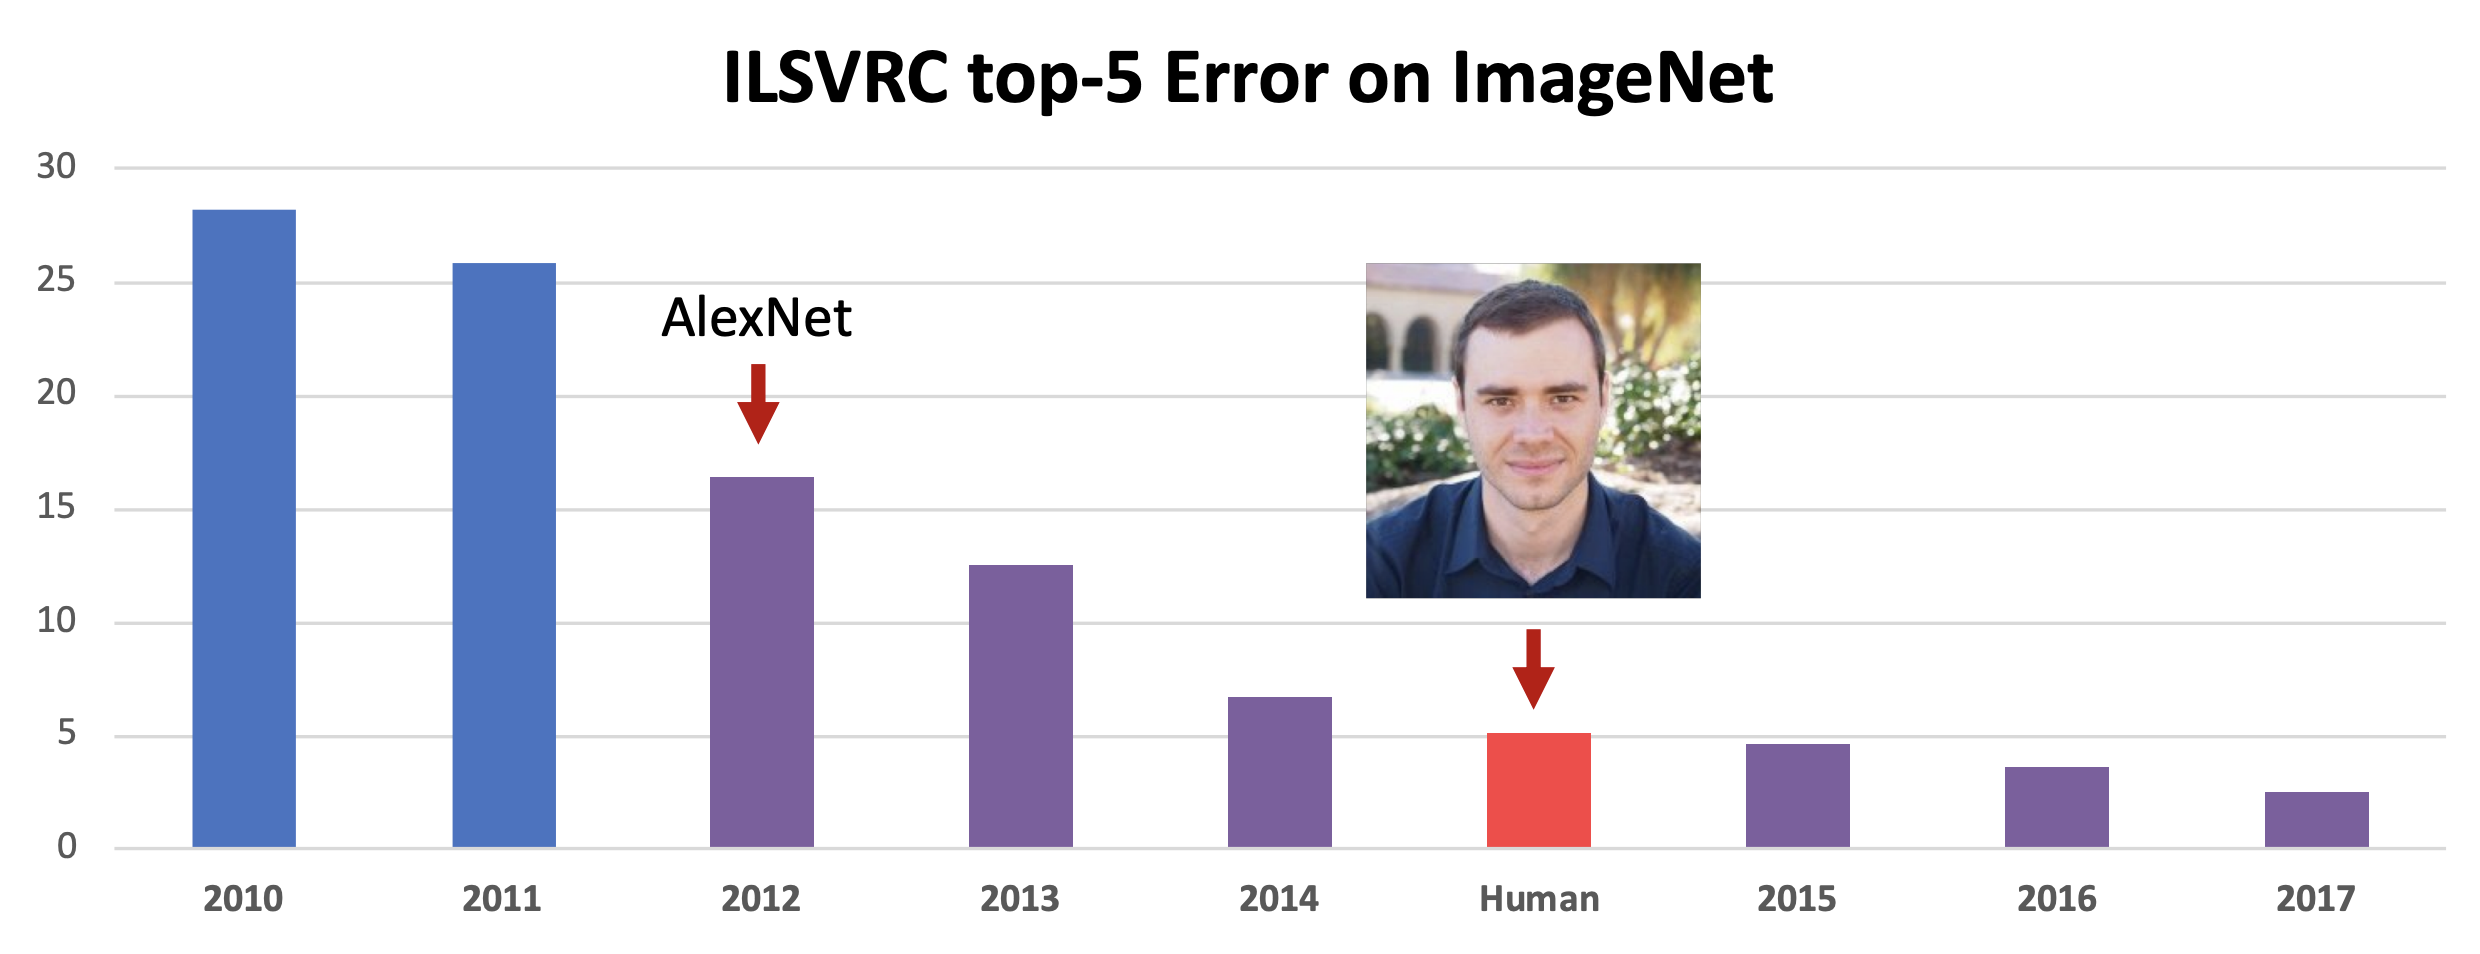
\includegraphics[width=0.8\linewidth]{images/image_net_perf.png}
    \end{figure}
    
    \item What does it mean to below the human bias ?
    \item Are we chasing the right metric ?
    \item Does it mean we can really trust these models in real environments ? when human safety is at stake ? (e.g. self-driving cars)
\end{itemize}
\end{frame}

\begin{frame}{Accuracy vs Robustness ?}
    \begin{figure}[H]
    \centering
    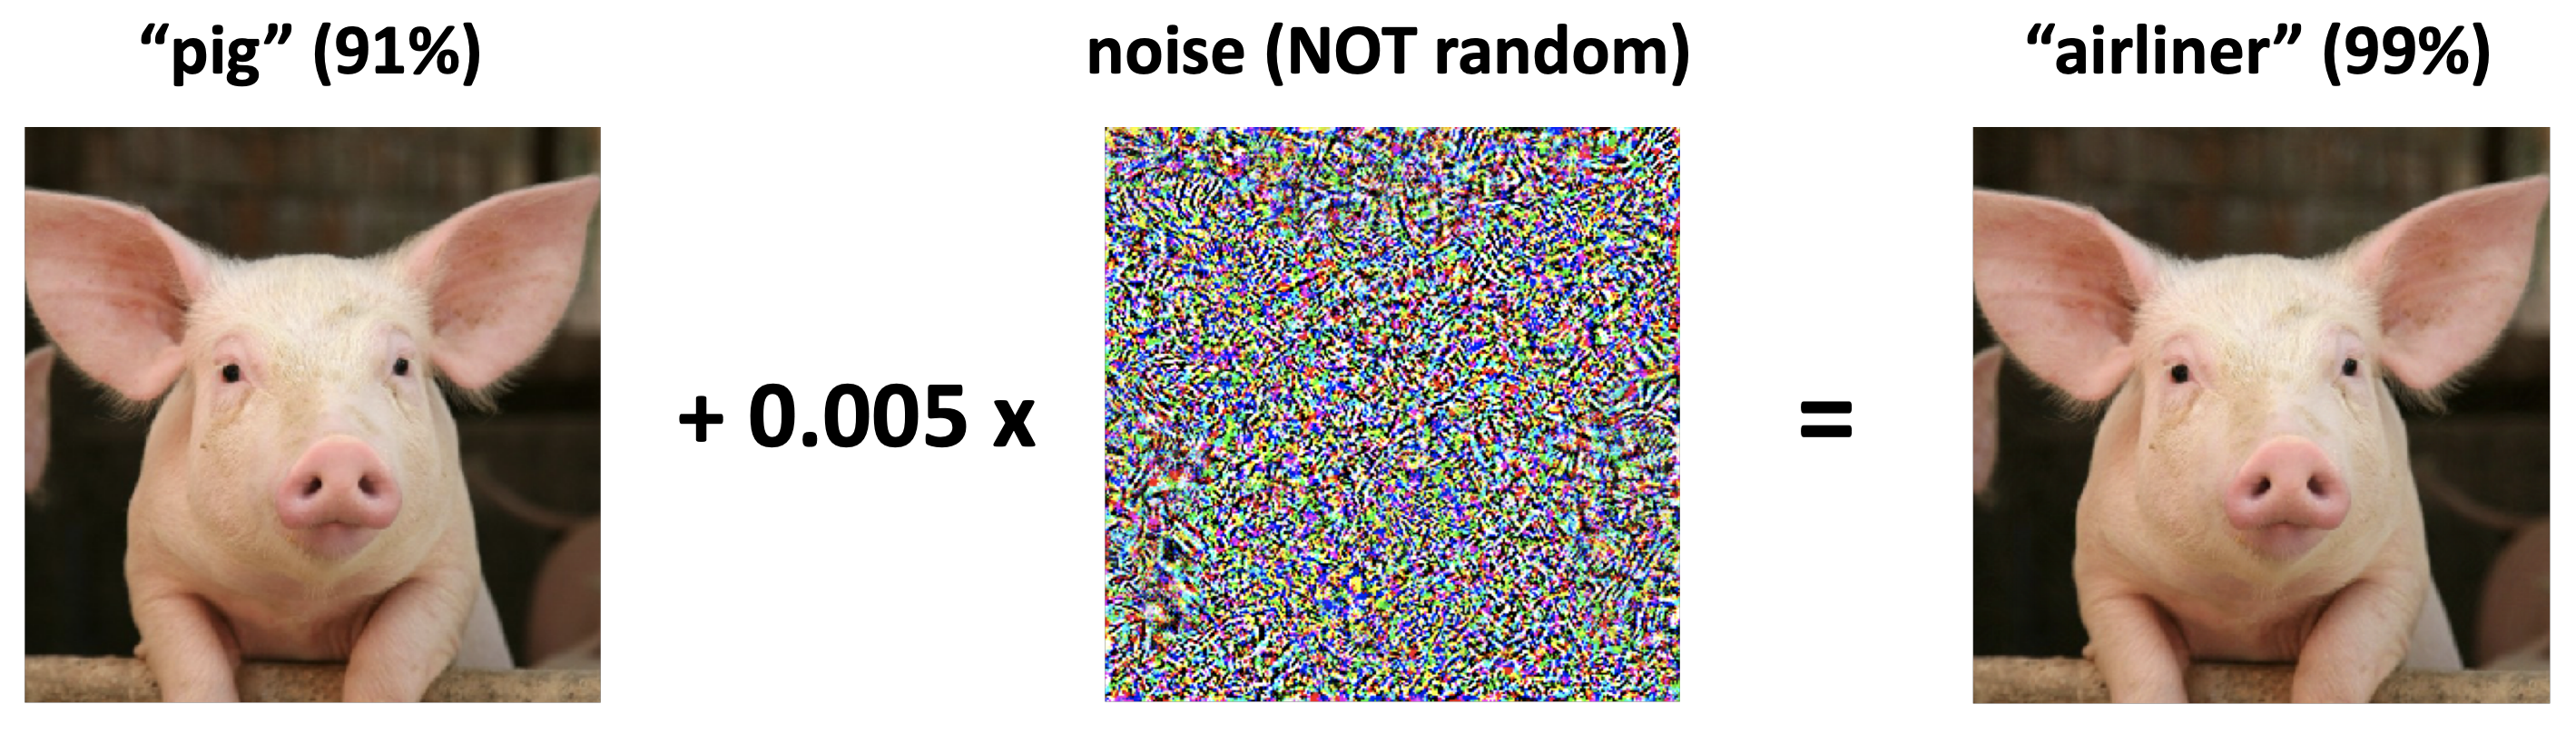
\includegraphics[width=0.8\linewidth]{images/pig_attack.png}
    \end{figure}
    
    \begin{figure}[H]
    \centering
    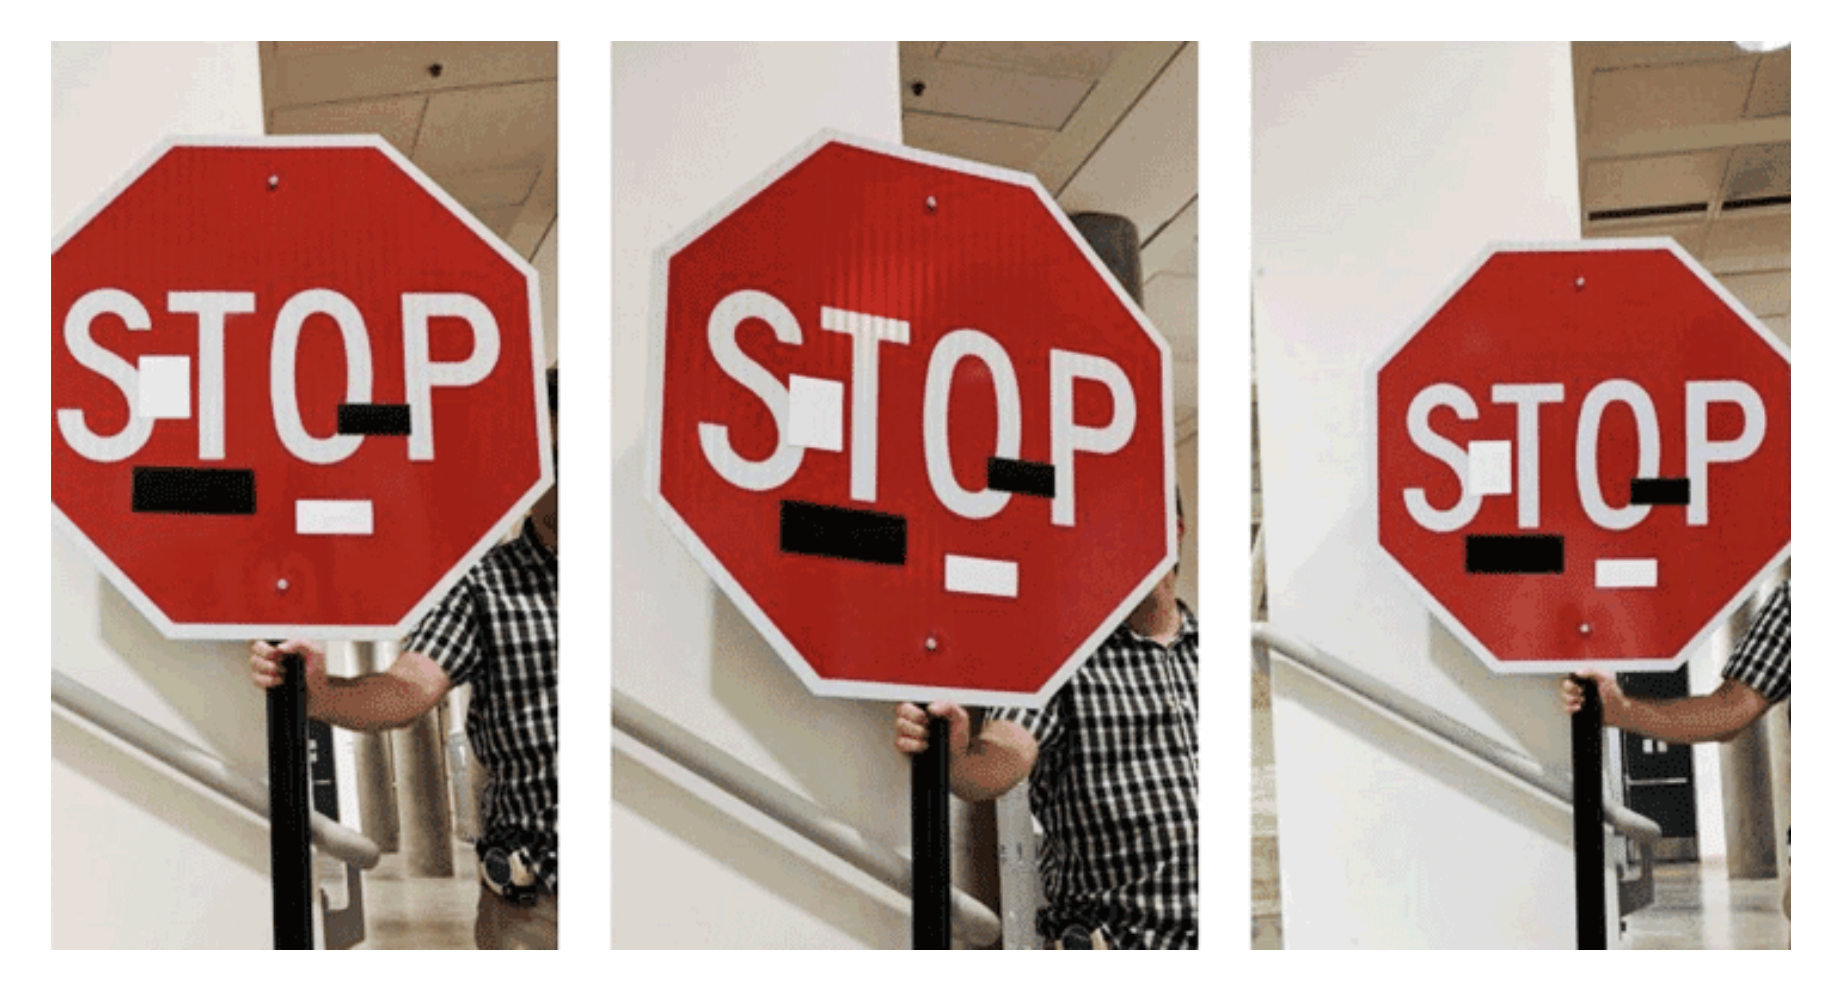
\includegraphics[width=0.6\linewidth]{images/stop_sign.png}
    \end{figure}
\end{frame}

\begin{frame}{A generalization / data issue ?}
    More generally, the assumption that train and test distribution are the same is wrong in general
    \begin{figure}[H]
    \centering
    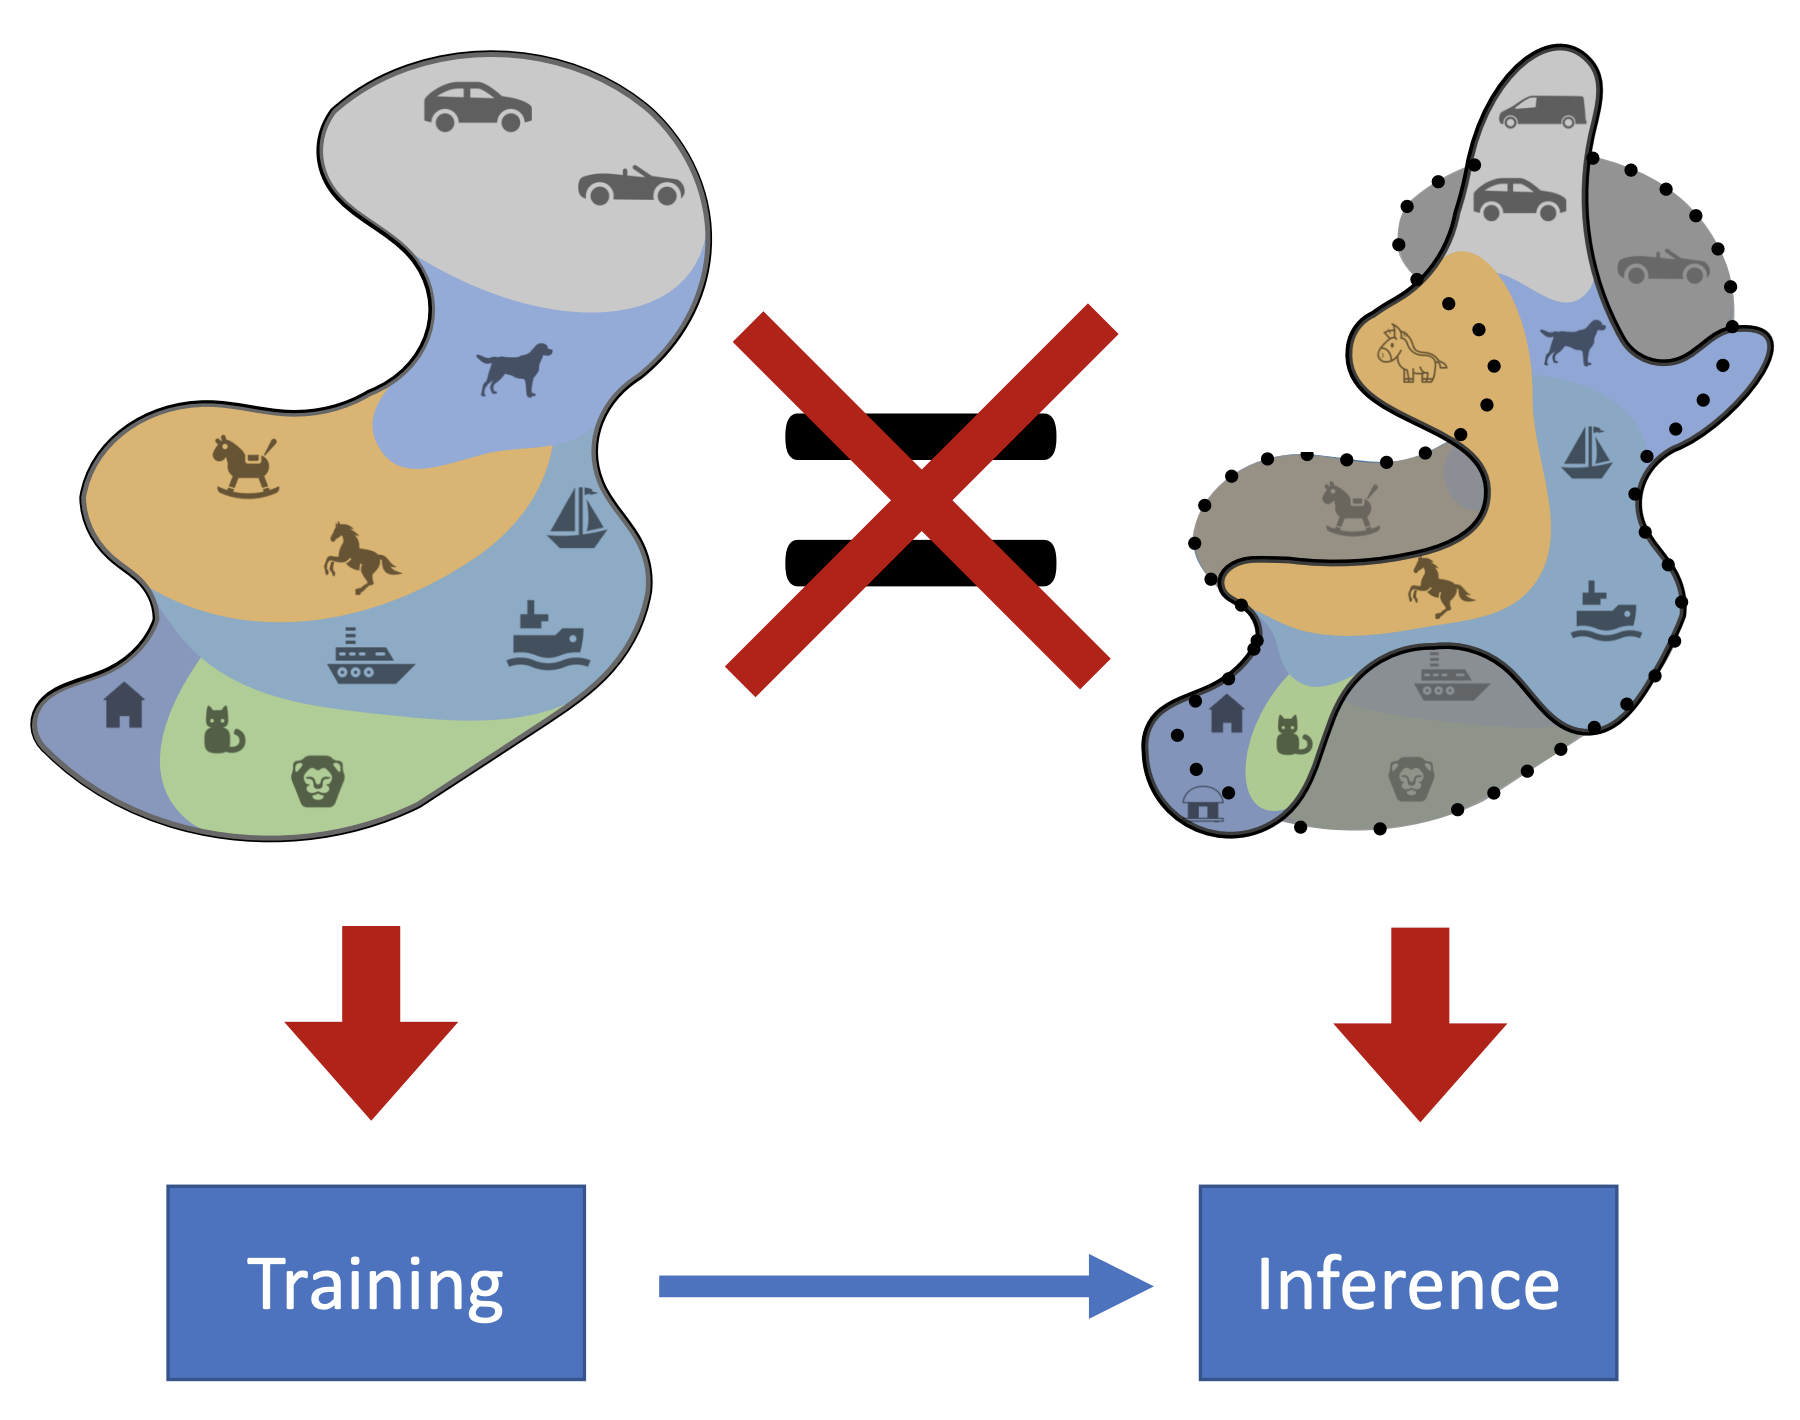
\includegraphics[width=0.6\linewidth]{images/distribution_mismatch.png}
    \end{figure}
    
    
\end{frame}

\section{Interpretation}

\begin{frame}{Maps}

\end{frame}

\section{Attacks and defenses}

\begin{frame}{SOTA Attacks}
    \begin{itemize}
        \item FGSM
        \item BIM
        \item DeepFool
        \item CW (\cite{carlini2017towards})
    \end{itemize}
\end{frame}

\begin{frame}{SOTA Defenses}
\begin{itemize}
    \item Defensive distillation (\cite{papernot2016distillation})
\end{itemize}
\end{frame}

\begin{frame}{SOTA Detection}

\begin{itemize}
    \item LID (\cite{ma2018characterizing})
    \item Mahalanobis (\cite{lee2018simple})
\end{itemize}

\end{frame}

\section{No free lunch ?}

\begin{frame}{No free lunch theorem ?}
Adversarial Accuracy

Accuracy

    \cite{dohmatob2018limitations}
\end{frame}

\section*{References}

\begin{frame}[allowframebreaks]\small
  \frametitle{References}
  \renewcommand*{\bibfont}{\footnotesize}
  \printbibliography
\end{frame}

\end{document}
